\documentclass[aspectratio=169]{../latex_main/tntbeamer}  % you can pass all options of the beamer class, e.g., 'handout' or 'aspectratio=43'
\usepackage{dsfont}
\usepackage{bm}
\usepackage[english]{babel}
\usepackage[T1]{fontenc}
%\usepackage[utf8]{inputenc}
\usepackage{graphicx}
\graphicspath{ {./figures/} }
\usepackage{algorithm}
\usepackage[ruled,vlined,algo2e,linesnumbered]{algorithm2e}
\usepackage{hyperref}
\usepackage{booktabs}
\usepackage{mathtools}

\usepackage{amsmath,amssymb}

\DeclareMathOperator*{\argmax}{arg\,max}
\DeclareMathOperator*{\argmin}{arg\,min}

\usepackage{amsbsy}
\newcommand{\vect}[1]{\bm{#1}}
%\newcommand{\vect}[1]{\boldsymbol{#1}}

\usepackage{pgfplots}
\pgfplotsset{compat=1.16}
\usepackage{tikz}
\usetikzlibrary{trees} 
\usetikzlibrary{shapes.geometric}
\usetikzlibrary{positioning,shapes,shadows,arrows,calc,mindmap}
\usetikzlibrary{positioning,fadings,through}
\usetikzlibrary{decorations.pathreplacing}
\usetikzlibrary{intersections}
\pgfdeclarelayer{background}
\pgfdeclarelayer{foreground}
\pgfsetlayers{background,main,foreground}
\tikzstyle{activity}=[rectangle, draw=black, rounded corners, text centered, text width=8em]
\tikzstyle{data}=[rectangle, draw=black, text centered, text width=8em]
\tikzstyle{myarrow}=[->, thick, draw=black]

% Define the layers to draw the diagram
\pgfdeclarelayer{background}
\pgfdeclarelayer{foreground}
\pgfsetlayers{background,main,foreground}

% Requires XeLaTeX or LuaLaTeX
%\usepackage{unicode-math}

\usepackage{fontspec}
%\setsansfont{Arial}
\setsansfont{RotisSansSerifStd}[ 
Path=../latex_main/fonts/,
Extension = .otf,
UprightFont = *-Regular,  % or *-Light
BoldFont = *-ExtraBold,  % or *-Bold
ItalicFont = *-Italic
]
\setmonofont{Cascadia Mono}[
Scale=0.8
]

% scale factor adapted; mathrm font added (Benjamin Spitschan @TNT, 2021-06-01)
%\setmathfont[Scale=1.05]{Libertinus Math}
%\setmathrm[Scale=1.05]{Libertinus Math}

% other available math fonts are (not exhaustive)
% Latin Modern Math
% XITS Math
% Libertinus Math
% Asana Math
% Fira Math
% TeX Gyre Pagella Math
% TeX Gyre Bonum Math
% TeX Gyre Schola Math
% TeX Gyre Termes Math

% Literature References
\newcommand{\lit}[2]{\href{#2}{\footnotesize\color{black!60}[#1]}}

%%% Beamer Customization
%----------------------------------------------------------------------
% (Don't) Show sections in frame header. Options: 'sections', 'sections light', empty
\setbeamertemplate{headline}{empty}

% Add header logo for normal frames
\setheaderimage{
	% 
\includegraphics[height=\logoheight]{figures/TNT_darkv4.pdf}
	
\includegraphics[height=\logoheight]{../latex_main/figures/luh_logo_rgb_0_80_155.pdf}
	% 
\includegraphics[height=\logoheight]{figures/logo_tntluh.pdf}
}

% Header logo for title page
\settitleheaderimage{
	% 
\includegraphics[height=\logoheight]{figures/TNT_darkv4.pdf}
	
\includegraphics[height=\logoheight]{../latex_main/figures/luh_logo_rgb_0_80_155.pdf}
	% 
\includegraphics[height=\logoheight]{figures/logo_tntluh.pdf}
}

% Title page: tntdefault 
\setbeamertemplate{title page}[tntdefault]  % or luhstyle
% Add optional title image here
%\addtitlepageimagedefault{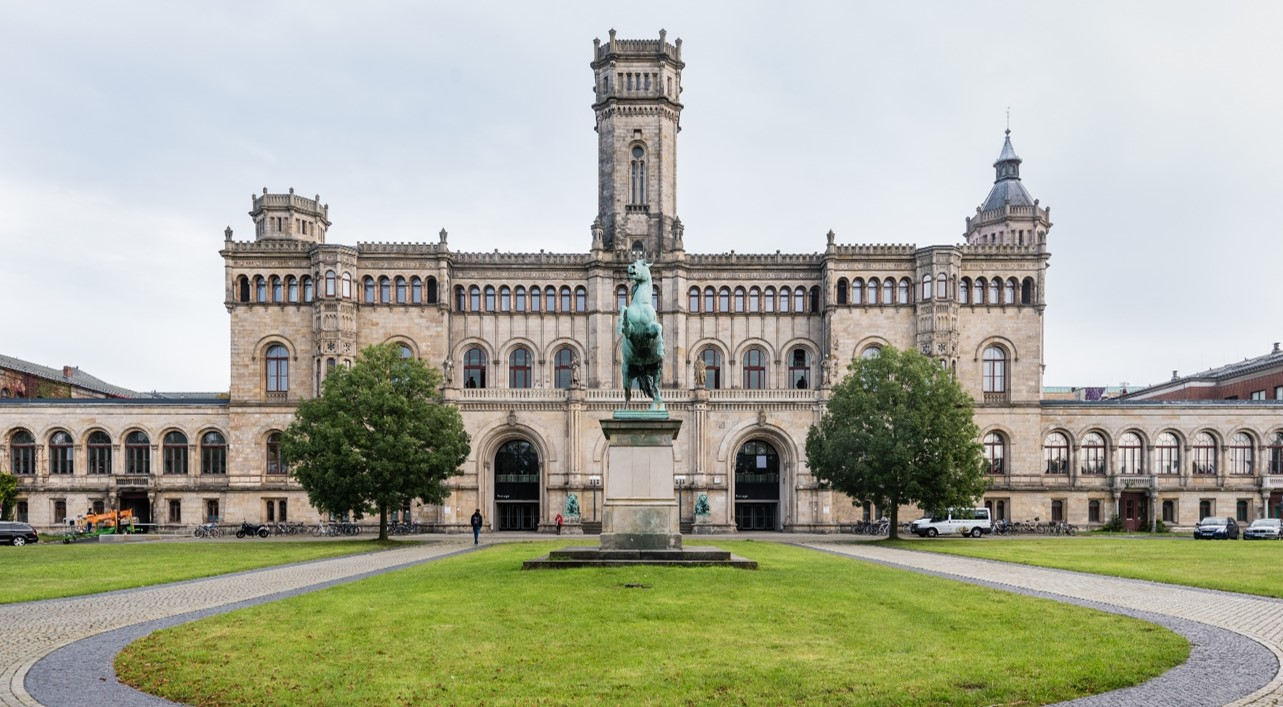
\includegraphics[width=0.65\textwidth]{figures/luh_default_presentation_title_image.jpg}}

% Title page: luhstyle
% \setbeamertemplate{title page}[luhstyle]
% % Add optional title image here
% \addtitlepageimage{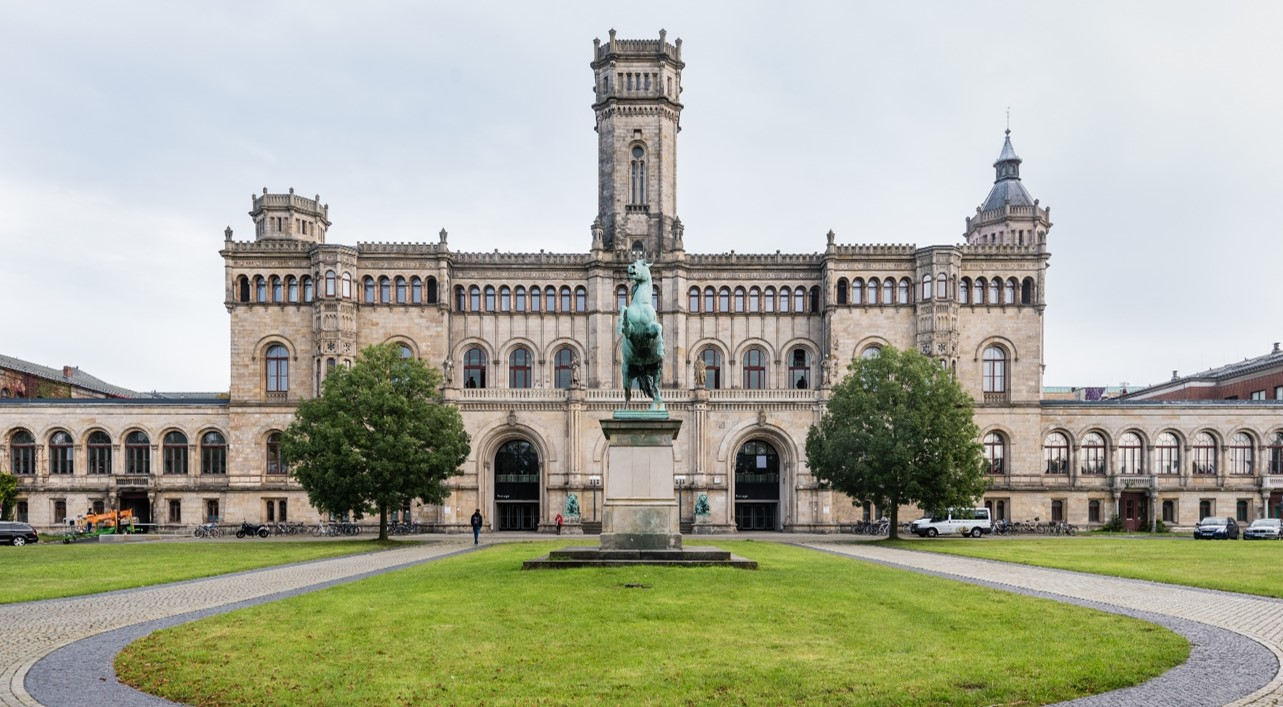
\includegraphics[width=0.75\textwidth]{figures/luh_default_presentation_title_image.jpg}}

\author[Abedjan \& Lindauer]{Ziawasch Abedjan \& Marius Lindauer\\[1em]
	
\includegraphics[height=\logoheight]{../latex_main/figures/luh_logo_rgb_0_80_155.pdf}\qquad
	
\includegraphics[height=\logoheight]{../latex_main/figures/DBIS_Kurzlogo.png}\qquad

\includegraphics[height=\logoheight]{../latex_main/figures/TNT_darkv4}\qquad

\includegraphics[height=\logoheight]{../latex_main/figures/L3S.jpg}	}
\date{Summer Term 2022; \hspace{0.5em} {
\includegraphics[height=1.5em]{../latex_main/figures/Cc-by-nc-sa_icon.svg.png}}; based on \href{https://ds100.org/fa21/}{[DS100]}
}


%%% Custom Packages
%----------------------------------------------------------------------
% Create dummy content
\usepackage{blindtext}

% Adds a frame with the current page layout. Just call \layout inside of a frame.
\usepackage{layout}


%%% Macros
%\renewcommand{\vec}[1]{\mathbf{#1}}
% \usepackage{bm}
%\let\vecb\bm

\title[Introduction]{DS: Logistic Regression, Part 1}
\subtitle{Logistic regression}

\graphicspath{ {./figure/} }
%\institute{}


\begin{document}
	
	\maketitle
	\begin{frame}{Linear vs. logistic regression}
	    In a linear regression model, we predict a quantitative variable (i.e., some real number) as a linear function of features.
	    \begin{itemize}
	        \item Our output, or response, y, could be any real number.
	    \end{itemize}
	    \begin{equation*}
	        \hat{y} = f_\theta (x) = x^T\theta
	    \end{equation*}
	    
	    In a logistic regression model, our goal is to predict a binary categorical variable (class 0 or class 1) as a linear function of features, passed through the logistic function.
	    \begin{itemize}
	        \item Our response is the probability that our observation belongs to class 1.
	        \item Haven’t yet done classification!
	    \end{itemize}
	    \begin{equation*}
	        \hat{y} =f_\theta (x) = P(Y=1|x) = \sigma (x^T\theta)
	    \end{equation*}
	\end{frame}
	
	
	\begin{frame}{Example calculation}
	   
	   \begin{columns}
	    
	   \begin{column}{.5\textwidth}
	    Suppose I want to predict the probability that LeBron’s shot goes in, given shot distance (first feature) and \# of seconds left on the shot clock (second feature).\\
	    \bigskip
	    I fit a logistic regression model using my training data, and somehow compute
	    \begin{equation*}
	        \hat{y}^T = [0.1 , -0.5]
	    \end{equation*}
	    
	   Under the logistic model, compute the probability his shot goes in, given that
	    \begin{itemize}
	        \item He shoots it from 15 feet.
	        \item There is 1 second left on the shot clock.
	    \end{itemize}
	    \end{column}
	    \begin{column}{.5\textwidth}
	        \begin{figure}
	            \centering
	            
\includegraphics[scale=.9]{Bild7}
	        \end{figure}
	    \end{column}
	    
	    \end{columns}
	\end{frame}
	
	
	\begin{frame}{Example calculation (solution)}
	   
	   \begin{columns}
	    
	   \begin{column}{.5\textwidth}
	   \begin{equation*}
	       x^T = [15, 1]\hspace{2cm} \hat{\theta}^T = [0.1, -0.5]
	   \end{equation*}
	   
	   \begin{align*}
	       P(Y=1|x) &= \sigma (x^T\hat{\theta})\\
	       &= \sigma (\hat{\theta}_1 \cdot \text{SHOT DISTANCE} + \hat{\theta}_2 \cdot \text{SECONDS LEFT} )\\
	       &=  \sigma (0.1 \cdot 15 + (-0.5) \cdot 1 )\\
	       &= \sigma (1)\\
	       &= \frac{1}{1 + e^{-1}}\\
	       &\approx 0.7311
	   \end{align*}
	    \end{column}
	    \begin{column}{.5\textwidth}
	        \begin{figure}
	            \centering
	            
\includegraphics[scale=.5]{Bild8}
	        \end{figure}
	    \end{column}
	    
	    \end{columns}
	\end{frame}
	
	
	\begin{frame}{Properties of the logistic function}
	   
	   \begin{columns}
	    
	   \begin{column}{.5\textwidth}
	   The logistic function is a type of sigmoid, a class of functions that share certain properties.
	   \begin{align*}
	       \sigma (t) = \frac{1}{1 + e^-t} \hspace{1cm} -\infty < t < \infty
	   \end{align*}
	   \begin{itemize}
	       \item Its output is bounded between 0 and 1, no matter how large t is.
	       \begin{itemize}
	           \item Fixes an issue with using linear regression to predict probabilities.
	       \end{itemize}
	       \item We can interpret it as mapping real numbers to probabilities.
	   \end{itemize}
	    \end{column}
	    \begin{column}{.5\textwidth}
	        \begin{figure}
	            \centering
	            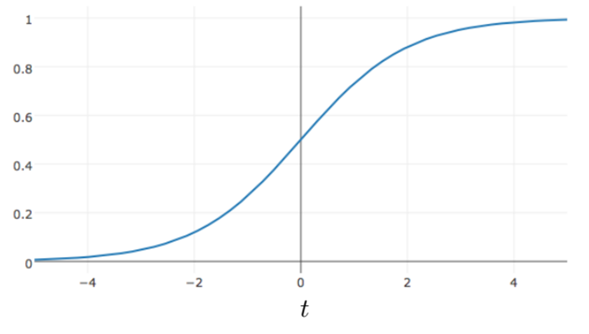
\includegraphics[scale=.65]{Bild9}
	        \end{figure}
	    \end{column}
	    
	    \end{columns}
	\end{frame}
	
	
	\begin{frame}{Properties of the logistic function}
	   %\begin{align*}
	   %    &\text{Definition}\\
	   %    &\sigma (t) = \frac{1}{1 + e{-t}} = \frac{e^t}{1+e^t} \hspace{2cm}\\
	   %    &\text{Range}\\
	   %    &0 < \sigma (t) < 1\\
	   %    &\text{Inverse}\\
	   %    & t = \sigma^{-1}(p) = log\left(\frac{p}{1-p}\right)\\
	   %    &\text{Reflection and Symmetry}\\
	   %    &1 - \sigma (t) = \frac{e^{-t}}{1 + e^{-t}} = \sigma (-t)\\
	   %    &\text{Derivative}\\
	   %    &\frac{d}{dt}\sigma \sigma (t) = \sigma (t)(1 - \sigma (t)) = \sigma (t)\sigma (-t)
	   %\end{align*}
	   \centering
        
\includegraphics[scale=.7]{Bild11}
	\end{frame}
	
	
	
	\begin{frame}{Shape of the logistic function}
	   
	   \begin{columns}
	    
	   \begin{column}{.5\textwidth}
	   Consider the plot of       $\sigma (\theta_1x)$      , for several different values of $\theta_1$. 
	   \begin{itemize}
	       \item If $\theta_1$ is positive, the curve increases to the right.
	       \item The further  $\theta_1$ is from 0, the steeper the curve.
	   \end{itemize}
	   In the notebook, we explore more sophisticated logistic curves.
	    \end{column}
	    \begin{column}{.5\textwidth}
	        \begin{figure}
	            \centering
	            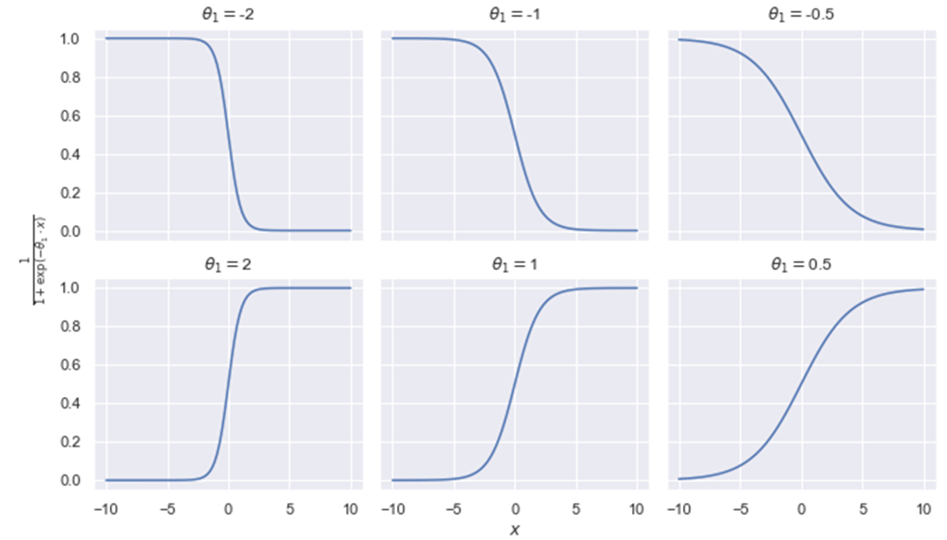
\includegraphics[scale=.3]{Bild10}
	        \end{figure}
	    \end{column}
	    
	    \end{columns}
	\end{frame}
	
	
	\begin{frame}{Parameter interpretation}
	   
	   Recall, we arrived at the model by assuming that the log-odds of the probability of belonging to class 1 was linear.
	   \begin{equation*}
	       P(Y=1|x) = \sigma(x^T\theta) \leftarrow log\left(\frac{P(Y=1|x)}{P(Y=0|x)}\right) = x^T\theta \leftarrow \frac{P(Y=1|x)}{P(Y=0|x)} = e^{x^T\theta}
	   \end{equation*}
	   $\frac{P(Y=1|x)}{P(Y=0|x)}$: This is the same as     $\frac{p}{1-p}$          , because
        \begin{equation*}
            P(Y=1|x) + P(Y=0|x) = 1
        \end{equation*}
        (Remember, we are dealing with binary classification – we are predicting 1 or 0.)
	\end{frame}
	
	
	\begin{frame}{Parameter interpretation}
	  Let’s suppose our linear component has just a single feature, along with an intercept term.
	   \begin{equation*}
	       \frac{P(Y=1|x)}{P(Y=0|x)} = e^{\theta_0 + \theta_1x}
	   \end{equation*}
	  What happens if you increase x by one unit?
	  \begin{itemize}
	      \item Odds is multiplied by $e^{\theta_1}$
	      \item If      $\theta_1$ > 0         , the odds increase.
	      \item If         $\theta_1$ < 0      , the odds increase.
	  \end{itemize}
	  What happens if              $x^T\theta = \theta_0 + \theta_1x = 0$?
	  \begin{itemize}
	      \item This means class 1 and class 0 are equally likely.
	      \item $e^0 = 1 \rightarrow \frac{P(Y=1|x)}{P(Y=0|x)} = 1 \rightarrow P(Y=1|x) = P(Y=0|x)$
	  \end{itemize}
	  The odds ratio can be interpreted as the “number of successes for each failure.”
	\end{frame}
\end{document}